\clearpage

\section{Introduction}

\subsection{Motivation}

In the age of digital documents, an author of content is confronted with the
question which document format to choose. Since every document format has its
advantages, one might not want to commit to a specific format to soon.

A series of blog posts might turn into a book or at least a pretty typeset
\emph{pdf}. An author might want to give the reader the freedom to read their
text on differently sized displays—if the reader has ever tried to read a paper
in \emph{pdf}-format on an e-book reader, no further motivation might be needed.

Luckily the problem of decoupling the initial document from output seems to be
solved by the rise of markup languages such as Markdown and alike. These types
of documents can be easily compiled into all sorts of output formats by programs
as \emph{Pandoc} \cite{pandoc}.

If the reader has no objections to such a publishing system, they might read no
further and write away their next \emph{format-agnostic} document. But if they
are interested in how they can easily extend the representation of their
document and let a type-checker reason about the \emph{well-formedness} of it,
they may find the findings gathered in this paper worth while.

\subsection{Type-safe extensibility}

This paper mostly outlines the ideas of the work on \emph{HSXML: Typed SXML}
\cite{hsxml} and the underlying idea of \emph{Finally Tagless Interpreters}
\cite{finally-tagless, finally-tagless-tut}.\\
The \emph{tagless-final style} is a solution to the expression problem
\cite{expression-problem}. It is closely related to the problem at hand, in that
it is concerned with the simultaneous extension of syntactic variants and
interpretations of them. This can be seen as an extensibility in two dimensions
[add schema like in Object-oriented programming versus abstract data types].

\subsection{?}

In short a \emph{tagless-final encoded} representation of documents like
\emph{HSXML} has in our opinion two major advantages over markup languages such
as Pandoc’s internal one:

\begin{enumerate}
\item Guarantee the well-formedness of the document by construction
\item Easy and full extensibility without loosing the guarantees of 1.
\end{enumerate}

While having these two advantages we still do not want to loose perspective and
solve to our initial goal:

\begin{enumerate}
\item Writing documents that are format agnostic—i.e. observe our source in
different ways
\end{enumerate}

or as described in the Wikipedia-article on \emph{Markup Languages}

\begin{quote}
Descriptive markup

Markup is used to label parts of the document rather than to provide specific
instructions as to how they should be processed. Well-known examples include
\LaTeX{}, HTML, and XML. The objective is to decouple the inherent structure of
the document from any particular treatment or rendition of it. Such markup is
often described as "semantic".
\end{quote}

\vspace*{\fill}
\begin{figure}
    \centering
    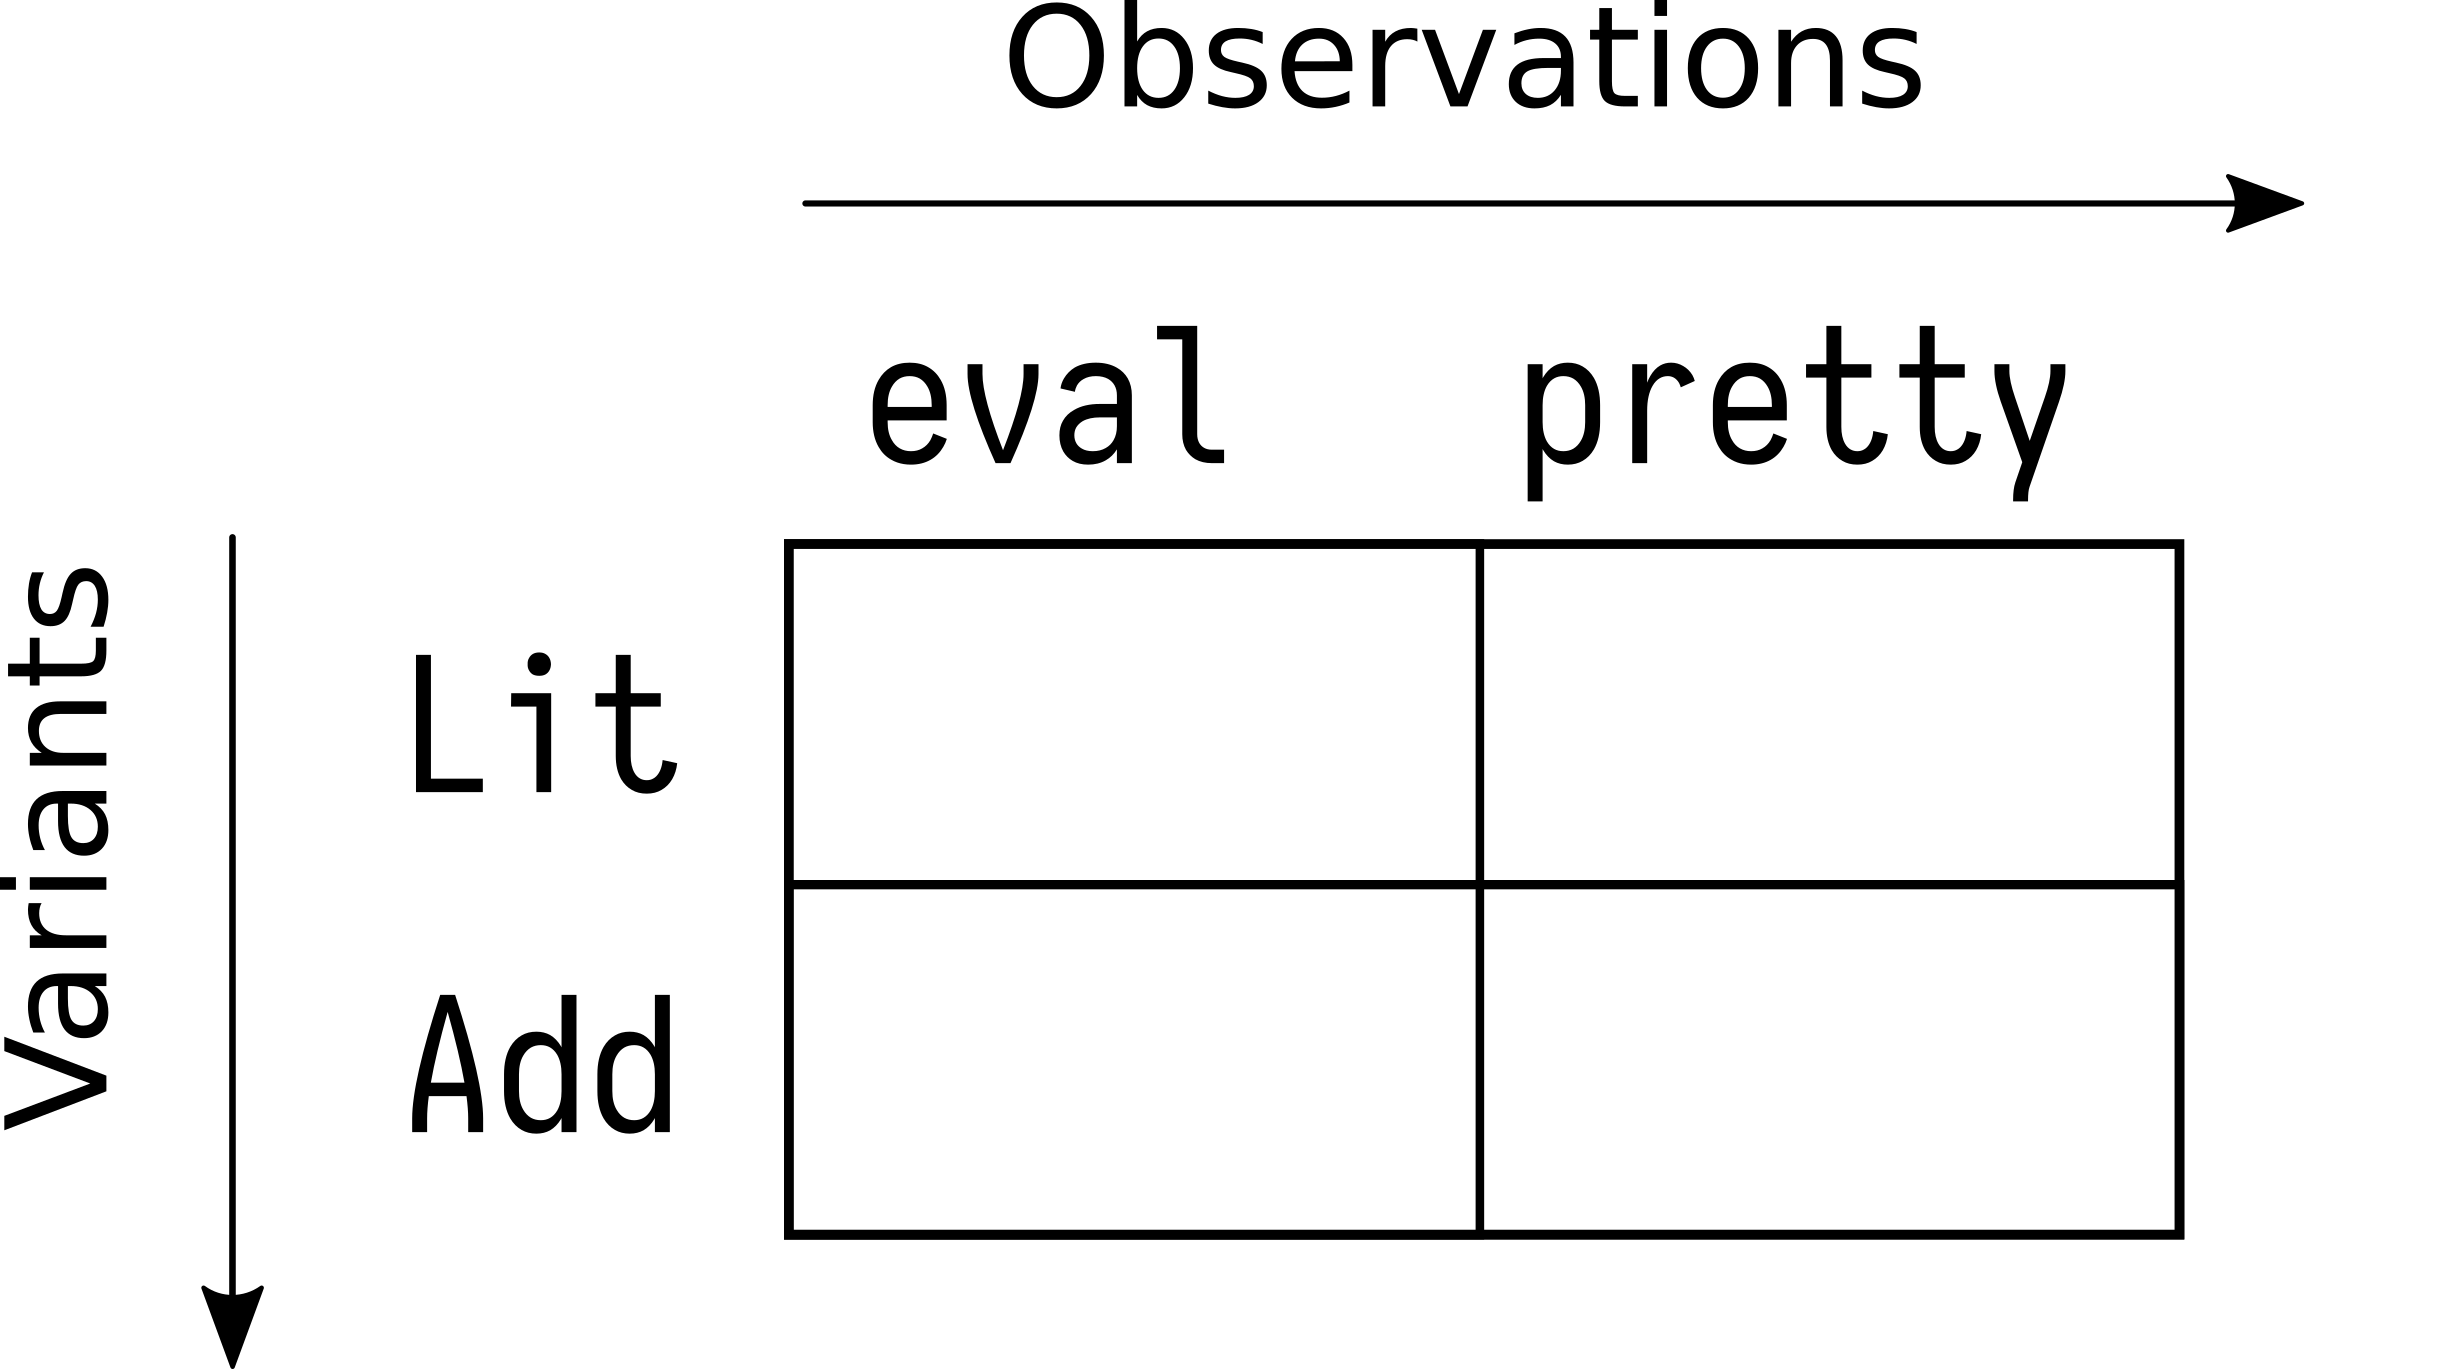
\includegraphics{resources/expression_problem_dimensions.png}
\captionof{figure}{\label{Expression_Problem}
Dimensions of the \emph{Expression Problem}}
\end{figure}
\vspace*{\fill}
\clearpage

\section{Extensibility of Markup Representations}
\subsection{Extensible Observers}

Pandoc achieves the separation of input and output format by choosing an
algebraic data type (ADT) as its intermediate representation. We will quickly
sketch why such an encoding leads to an easy extensibility of constructors by
looking a subset of Pandoc's abstract syntax tree (AST) and writing some
\emph{observers} for it.

Given the representation (Figure \ref{Pandoc_AST}) we can write observers that
interpret this data in different ways (Figure \ref{Pandoc_Views}). So in the
dimension of observers an ADT encoding is obviously extensible.

Now we can construct a tree in the host language and interpret it in two
different ways:
\begin{lstlisting}
groceryList :: [Block]
groceryList
  = [ Heading 1  [ Str "Grocery list"]
    , BulletList [ Paragraph [ Str "1 Banana"]
                 , Paragraph [ Str "2 "
                             , Emph [Str "organic"]
                             , Str " Apples"]]]

groceryListCM :: Markdown
groceryListCM = mconcatMap docToCMark groceryList

groceryListLaTeX :: LaTeX
groceryListLaTeX = mconcatMap docToLaTeX groceryList
\end{lstlisting}

We can make our life a bit easier by adding an instance for \texttt{IsString}
for our representation. This injects \texttt{String} automatically into our data
types by applying \texttt{fromString} to it.

\begin{lstlisting}
instance IsString Inline where
  fromString = Str
\end{lstlisting}


Our initial definition is now even more concise:

\begin{lstlisting}
groceryListShort :: [Block]
groceryListShort
  = [ Heading 1  [ "Grocery list"]
    , BulletList [ Paragraph ["1 Banana"]
                 , Paragraph ["2 ", Emph ["organic"], " Apples"] ]]
\end{lstlisting}

\begin{figure}
\begin{lstlisting}
data Block
  = Paragraph   [Inline] -- ^ Paragraph
  | BulletList  [Block]  -- ^ Bullet list (list of items, each a block)
  | Heading Int [Inline] -- ^ Heading - level (int) and text (inlines)
  
data Inline
  = Str String      -- ^ Text (string)
  | EmDash          -- ^ em dash
  | Emph   [Inline] -- ^ Emphasized text (list of inlines)
  | Strong [Inline] -- ^ Strongly emphasized text (list of inlines)
\end{lstlisting}
\captionof{figure}{\label{Pandoc_AST}
This is part of Pandoc’s ADT-encoded AST modulo \texttt{EmDash}}
\end{figure}

\begin{figure}
\begin{lstlisting}
docToCMark :: Block -> Markdown
docToCMark (Paragraph text)     = mconcatMap inlineToCMark text
docToCMark (BulletList docs)    = addLineBreak $ mconcatMap (mappend "- " . docToCMark) docs
docToCMark (Heading level text) = addLineBreak $ headingPrefix `mappend` mconcatMap inlineToCMark text
 where
  headingPrefix = mconcat $ replicate level "#"

addLineBreak :: Markdown -> Markdown
addLineBreak text = text `mappend` "\n"

inlineToCMark :: Inline -> Markdown
inlineToCMark (Str content)     = fromString content
inlineToCMARK (Emph contents)   = "*" `mappend` mconcatMap inlineToCMark contents `mappend` "*"
inlineToCMARK (Strong contents) = "**" `mappend` mconcatMap inlineToCMark contents `mappend` "**"
inlineToCMARK EmDash            = "---"

docToLaTex :: Block -> LaTeX
...

inlineToLaTex :: Inline -> LaTeX
...

deleteme$
\end{lstlisting}
\captionof{figure}{\label{Pandoc_Views}
Observers of ADT encoding}
\end{figure}

\clearpage

\subsection{Extensible Variants}

The simple ADT encoding works very well, as long as we have foreseen every
variant we might want to create. But as soon as we want to add a new kind of
variant—e.g. a node representing the em dash—we are out of luck. Even if we
have access to the original ADT-definition and we could add this new variant,
this would break all existing observers that were written for the original set
of variants.

\subsection{Relationship to the Expression Problem}

To be extensible in the dimension of observers as well as the dimension of the
variants—while still guaranteeing statically their compatibility—is quite a
challenge and one that is common when writing software. It was coined as the
\emph{Expression Problem} by Wadler \cite{expression-problem} and many solutions
have been proposed.

The most prominent solutions—that are widely used the Haskell-ecosystem—are
described in \emph{Data-types a la carte} \cite{data-types-a-la-carte} and in
\emph{Finally Tagless, Partially Evaluated} \cite{finally-tagless}. Kiselyov’s
et al. solution to this is, in our opinion, both easy to use and the notation
for constructing AST is extremely similar to the ADT-encoded one.


\section{Simple Tagless-Final Encoding}

Our first attempt to encode our document in the tagless-final encoding will not
have the distinction between \texttt{Doc} and \texttt{Inline}—which was enforced
by the Pandoc-encoding. But later we will see that we are able to recover that
property quite easily with great extensibility properties.

The basic idea of the TF encoding is as follows:

\begin{itemize}
\item Create a type class that specifies all our constructors in Church [add
  footnote with Böhm Berarducci citation] encoding (Figure \ref{First_Step_FT})
\item Parametrize over the return-type and recursive fields of those
  constructors (Figure \ref{Second_Step_FT})
\end{itemize}

\begin{figure}
\begin{lstlisting}
data Doc = Doc String

instance Monoid (Doc doc) where
  mappend (Doc doc1) (Doc doc2) = Doc $ doc1 `mappend` doc2
  mempty = Doc mempty

-- Constructors

class Block where
  paragraph  ::        [Doc] -> Doc
  bulletList ::        [Doc] -> Doc
  heading    :: Int -> [Doc] -> Doc

class Inline a where
  emDash ::           Doc
  str    :: String -> Doc
  str = Doc
\end{lstlisting}
\captionof{figure}{\label{First_Step_FT}
First Step FT-encoding}
\end{figure}

\begin{figure}
\begin{lstlisting}
-- DocConstraint defined using ConstraintKinds
type DocConstraint doc = (Monoid doc, IsString doc)

newtype Doc doc = Doc doc

instance DocConstraint doc => -- Have to restrict for the use of 'mempty'
  Monoid (Doc doc) where
  mappend (Doc doc1) (Doc doc2) = Doc $ doc1 `mappend` doc2
  mempty = Doc mempty

-- Constructors

class Block a where
  paragraph  ::        [Doc a] -> Doc a
  bulletList ::        [Doc a] -> Doc a
  heading    :: Int -> [Doc a] -> Doc a

class DocConstraint a =>
  Inline a where
  emDash ::           Doc a
  str    :: String -> Doc a
  str = Doc . fromString
\end{lstlisting}
\captionof{figure}{\label{Second_Step_FT}
Second Step FT-encoding}
\end{figure}

The type classes look basically like a GADT-encoding where all recursive
occurrences and the return-type are parametrized over.

The observers will now be instances of theses type classes. The reader might
notice that we cannot use the same carrier type for different interpretations of
our AST—otherwise we would get overlapping instances. This can be quite easily
solved by wrapping the carrier type into a \emph{newtype} and add or derive the
needed instances for it. In our case \texttt{Markdown} is simply a
\emph{newtype} of \texttt{String}. Therefore the instances for \texttt{IsString}
and \texttt{Monoid} are straightforward to implement.

Figure \ref{FT_Observer} shows the implementation of an observer in the
tagless-final encoding. The implementation is really similar the one in the ADT
encoding. But if we have close look, we can see that—since our data type is
Church encoded—the observers do not need to be called recursive explicitly. This
makes both our code simpler and is essential for extensibility.

\begin{figure}
\begin{lstlisting}
-- Implement Markdown observer

instance Block Markdown where
  paragraph = fromInline . mconcat
  bulletList = addLineBreak . mconcat . map (mappend (fromInline "\n- "))
  heading level = addLineBreak . fromInline . mappend (mconcat $ replicate level "#") . mconcat

addLineBreak :: DocAtts doc => DocWithCtx ctx doc -> DocWithCtx ctx doc
addLineBreak (DocWithCtx doc) = DocWithCtx $ doc `mappend` "\n"

instance Inline Markdown where
  emDash = "---"

instance Styles Markdown where
  emph   texts = "*"  `mappend` mconcat texts `mappend` "*"
  strong texts = "**" `mappend` mconcat texts `mappend` "**"


-- Implement LaTeX observer

instance Block LaTeX where
...

instance Inline LaTeX where
...

instance Styles LaTeX where
...
\end{lstlisting}
\captionof{figure}{\label{FT_Observer}
Observer implementation in the tagless-final encoding}
\end{figure}


\clearpage

Let's see how our example from above looks in our new encoding:

\begin{lstlisting}
groceryList
  = [ heading 1  [str "Grocery list"]
    , bulletList [ paragraph [ str "1 Banana"]]
                 , paragraph [ str "2 "
                             , emph [str "fresh"]
                             , str " Apples"] ]
\end{lstlisting}


As before, we can automate the injection of \texttt{String} into our encoding by
using the \texttt{OverloadedStrings} language pragma. We do this be adding a
constraint on the type classes, so every output format (i.e. carrier type) must
have an \texttt{IsString} instance.

Interestingly \texttt{Doc} has now no dependency on \texttt{Inline} anymore and
we are now allowed to create the following AST:

\begin{lstlisting}
badHeading = [ heading 1  [ heading 2 [str "Headingception!!"] ] ]
\end{lstlisting}

As noted above, we lost the distinction between \texttt{Doc} and
\texttt{Inline}. But we also gained something—\emph{Doc} can now be used
without \emph{Inline} and we can now also add new variants without changing our
original variant definitions:

\begin{lstlisting}
class Styles doc where
  emph   :: [DocWithCtx InlineCtx doc] -> DocWithCtx InlineCtx doc
  strong :: [DocWithCtx InlineCtx doc] -> DocWithCtx InlineCtx doc
\end{lstlisting}

Not only can we now mix those node types at will, but the type of an expression
will reflect which type classes (i.e. algebras) we used for constructing it:

\begin{lstlisting}
stylishNote :: (Inline a, Styles a) => a
stylishNote = strong [str "Green Tea keeps me awake"]
\end{lstlisting}

That is why the type system can now statically tell us whether we can evaluate
\texttt{stylishNote} to a particular type.

If we wanted to evaluate an expression, that uses constructors that belong to a
type class \emph{X} and we would want to evaluate the expression to some carrier
type \emph{C}, \emph{C} has to be instance of \emph{X}. Since this is a static
property, it can be decided at compile time.

\subsection{A short note on GHC’s Type Inference}

When we define an AST like \texttt{stylishNote} GHC’s type inference might come
in our way. If no type signature for \texttt{stylishNote} is supplied GHC will
try to infer a concrete type for this definition and not the most generalized
type.

We can avoid this by either supplying the generalized type signature—as done
above—or using the language pragma \emph{NoMonomorphismRestriction}.

\section{Recover Context Awareness}

To regain the context awareness of the Pandoc encoding, we add another field
named \texttt{ctx} to our \texttt{Doc} wrapper (Figure \ref{ContextWrapper}).
\texttt{ctx} is a phantom type and with its help we can specify in which
context a constructor can be used. Since phantom types are not materialized on
the value level, we are simply using empty data declarations as context types.

\begin{lstlisting}
-- Context definitions
data InlineCtx
data BlockCtx
\end{lstlisting}

As shown before, the first tagless-final encoding had the disadvantage, that we
could construct a heading inside another heading. To prohibit this, the
\texttt{heading} constructor has the following context-aware definition:

\begin{lstlisting}
class Block doc where
  heading :: Int -> [DocWithCtx InlineCtx doc] -> DocWithCtx BlockCtx doc
  ...
\end{lstlisting}

The type signature states, that the function expects a
\texttt{DocWithCtx}-wrapper in the \texttt{InlineCtx}-context and returns a
wrapper in the \texttt{BlockCtx}-context. With this refined signature a heading
inside a heading will be rejected by the type system.

To convince Haskell’s type system that a conversion from \texttt{InlineCtx} to
\texttt{BlockCtx} is possible, we can use the following type class:

\begin{lstlisting}
class FromInline ctx where
  fromInline :: DocWithCtx InlineCtx doc -> DocWithCtx ctx doc
  fromInline (DocWithCtx doc) = DocWithCtx doc

instance FromInline BlockCtx
\end{lstlisting}


The set of available contexts should be defined generously, since all
independent extensions of the AST should agree on them. This is obviously are
restriction—but one that is intended.

It is also possible to create context independent constructors. This can be
achieved by parametrizing over the context:

\begin{lstlisting}
class Math doc where
  qed :: DocWithCtx ctx doc
\end{lstlisting}

\begin{figure}[t]
\begin{lstlisting}
newtype DocWithCtx ctx doc = DocWithCtx doc
\end{lstlisting}
\captionof{figure}{\label{ContextWrapper}
Context-aware wrapper}
\end{figure}

\section{Conclusion}

We presented two different encodings that we can choose from for representing a
markup language. While the ADT encoding might look like the tool for the job, we
have seen that it has some serious limitations. If we do not want to commit to a
set of variants forever and do not want to break other people's observers by
changing the ADT definition—the tagless-final approach might be a good solution
also for this instance of the \emph{Expression Problem}.

For those who want to study this approach in more depth—the lecture notes on
\emph{Typed Tagless Final Interpreters} \cite{finally-tagless-tut} are a great
resource.
